\chapter{Analyse}
In diesem Kapitel werden die in Kapitel \ref{ch:konzeption} vorgestellten Systeme analysiert.

\section{128MB Konfigurationen}
Zunächst werden alle Tests gegen die 128MB Konfigurationen ausgeführt. In den folgenden Sektionen wird dann die Speicher- und Prozessorgröße erhöht. 

\subsection{Pipe-Clean Tests}
Zunächst wird die Performance der SUTs in der bestmöglichen Situation mit einem einzigen Nutzer ermittelt. Ziel dessen ist es, eine Vergleichsgrundlage für die darauf folgenden Tests zu schaffen. Der Test wurde mit einer Dauer von zehn Minuten mit einem aktiven Benutzer für jeden Use-Case durchgeführt. Jeder Test wurde drei mal ausgeführt und die Metriken über die Gesamtmenge der Daten aggregiert. Bei den Requests wurde die Summe gebildet, bei den durchschnittlichen Requests pro Sekunde das arithmetische Mittel.

\begin{figure}[H]
    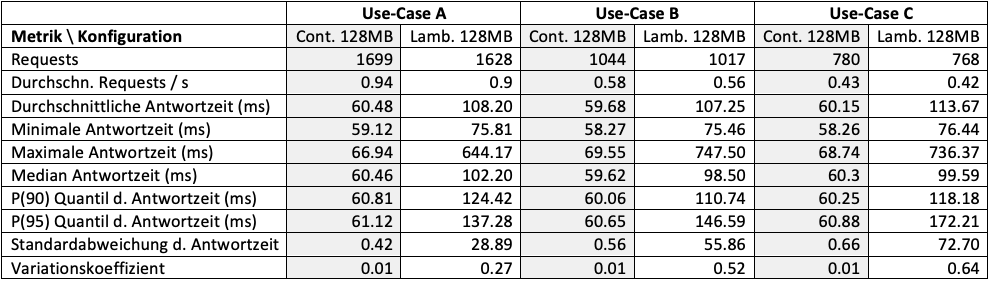
\includegraphics[width=\textwidth]{img/pipe128-comparison.png}
    \caption[Vergleich der Pipe-Clean Tests für 128MB]{Vergleich der Pipe-Clean Tests für 128MB}
    \label{fig:pipe128-comparison}
\end{figure}

Abbildung \ref{fig:pipe128-comparison} zeigt die Ergebnisse des Tests für die Funktionen mit 128MB CPU bzw. RAM. Die Zahlen sind aufgrund des Tests-Tools mit der Englischen Notation mit Punkt anstatt eines Kommas angegeben. Es ist zu erkennen, dass die Container Anwendung in allen Fällen eine deutlich geringere Antwortzeit als die Lambda Anwendung aufweist. Im Median ist der Container bei Use-Case A etwa 41,74ms schneller als die Lambda-Funktion. Während die maximale Antwortzeit bei ersterer nur etwa 10,7\% über dem Median liegt, ist sie bei der Lambda-Funktion etwa 630\% über ihrem Median. Dass die Lambda-Anwendung eine überaus große Varianz in ihren Antwortzeiten aufweist, wird auch in ihrer Standardabweichung von bis zu 72ms deutlich, währende sie bei der Container Anwendung in allen drei Use-Cases unter 1ms liegt. Interessanterweise liegt die Antwortzeit der Lambda-Anwendung im Median in allen drei Use-Cases bei ähnlichen Werten um ca. 100ms. Andererseits nimmt die Standardabweichung und das P(95) Quantil der Antwortzeit bei Use-Case B im Vergleich zu Use-Case A deutlich zu. Und auch bei Use-Case C ist ein deutlicher Anstieg der Werte zu beobachten. Vermutlich ist dies auf die größere Anzahl an angefragten Endpunkten zurückzuführen, da dadurch mehr Coldstarts durchgeführt werden müssen. Auch bei der Container-Anwendung ist keine Veränderung der Median-Antwortzeit um ca. 60ms festzustellen. Die Standardabweichung der Antwortzeit erhöhte sich nur leicht von 0,42 auf 0,66. Der Variationskoeffizient blieb aber in allen drei Use-Cases bei 0,01.

Anhand der Vergleichstabelle lassen sich auch Erkenntnisse über die einzelnen Use-Cases ableiten. Use-Case A setzt sowohl bei der Container- als auch bei der Lambda-Anwendung deutlich mehr Requests in der Sekunde ab als es bei den Use-Cases B und C der Fall ist. Dies liegt an der größeren Think-Time von 3 Sekunden, wie sie bei den Use-Cases mit Benutzer-Eingaben zum Einsatz kommt.

\subsection{Stress-Tests}
Um RQ1 zu beantworten, muss zunächst die maximale Auslastung eines einzelnen Containers ermittelt werden. Dazu wurden mehrere Stress-Tests durchgeführt. Ein Stress-Test dient dazu, die Grenzen des SUTs herauszufinden. Da Lambda ein von Natur aus automatisch horizontal skalierendes System ist, werden die Test zunächst für die Container-Anwendung durchgeführt und im Anschluss die Lambda-Anwendung mit der gleichen Test-Konfiguration getestet. Die Anzahl der VUs wird bei den Stress-Tests wie von Molyneaux\cite{molyneaux_art_2014} empfohlen immer stufenweise erhöht. Das bedeutet, dass nach jedem Ramp-Up (ein linearer Anstieg) eine gleichlange Periode mit einer konstanten Anzahl an Benutzern folgt. Abbildung \ref{fig:stress-vus-example} verdeutlicht dies anhand eines Stress-Tests, bei dem bis zu 600 gleichzeitige Virtuelle Benutzer erstellt werden. In 60 Sekunden Zeitabschnitten werden nach und nach immer 60 Benutzer hinzugefügt. Daraufhin folgt eine weitere 60 Sekunden lange Periode, in der die Anzahl der VUs nicht weiter erhöht wird. Der gesamte Test hat demnach eine Dauer von 40 Minuten. Eine Cooldown-Phase nach den vollen 600 Benutzern wird hier nicht eingelegt, da das Skalierungsverhalten nicht untersucht wird.

\begin{figure}[H]
    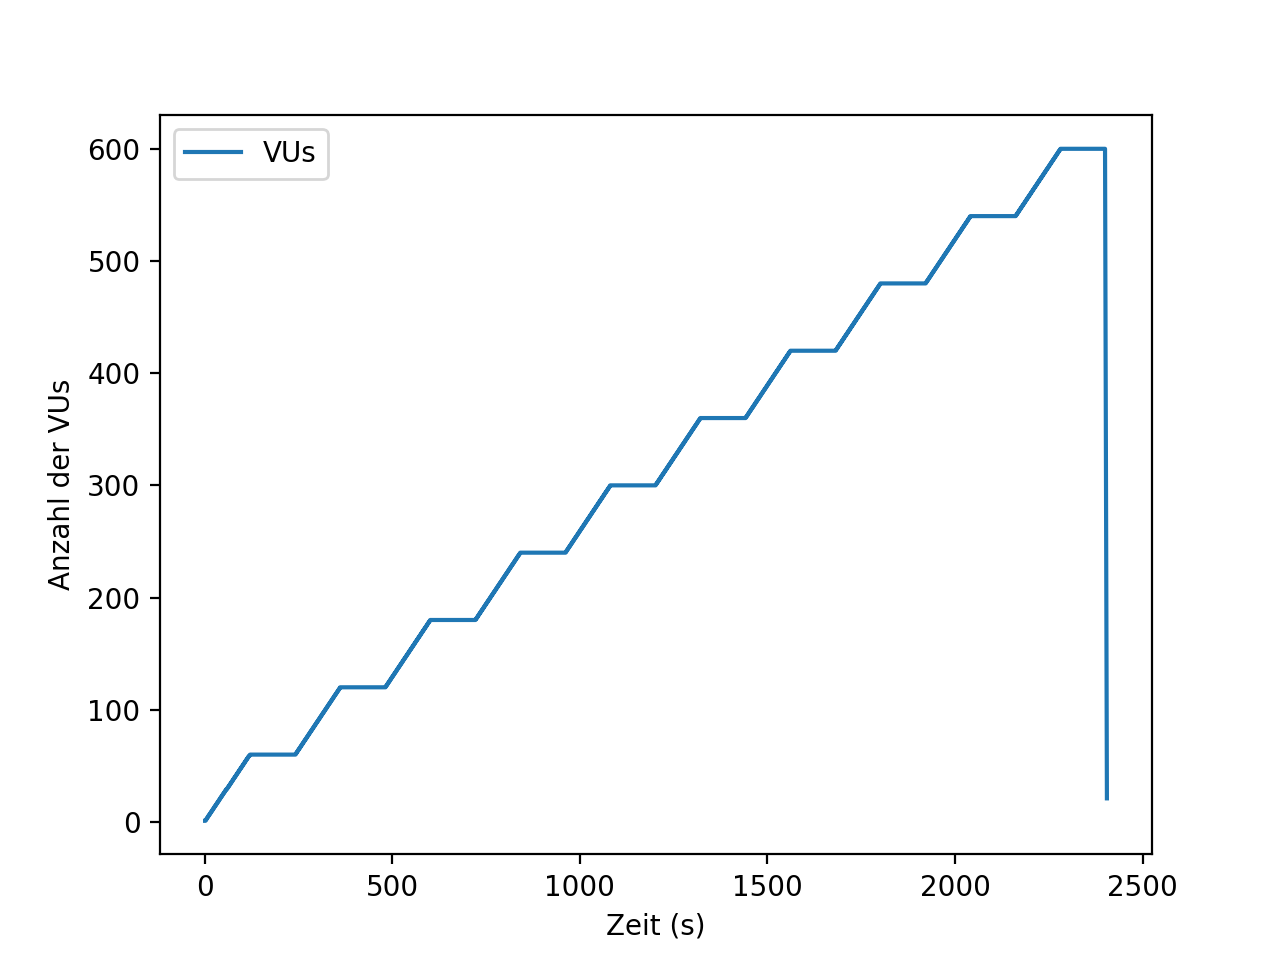
\includegraphics[width=\textwidth]{img/stress-vus-example.png}
    \caption[Beispiel-Anstieg der gleichzeitigen VUs für einen Stress Test]{Beispiel-Anstieg der gleichzeitigen VUs für einen Stress Test}
    \label{fig:stress-vus-example}
\end{figure}

\subsubsection{Container}
Für die containerisierte Anwendung in der 128MB Konfiguration wurden mehrere Stress-Tests durchgeführt, bis das Limit der gleichzeitigen Benutzer identifiziert werden konnte. Abbildung \ref{fig:fargate128-stress-comparison} zeigt die getesteten Use-Cases und die Stress-Test Konfiguration. 

\begin{figure}[H]
    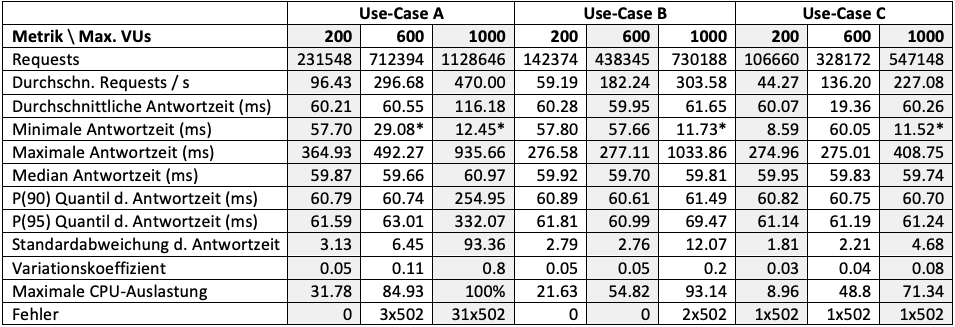
\includegraphics[width=\textwidth]{img/fargate128-stress-comparison.png}
    \caption[Fargate 128MB Stress-Test Vergleich]{Fargate 128MB Stress-Test Vergleich}
    \label{fig:fargate128-stress-comparison}
\end{figure}

Der erste Test wurde mit bis zu 200 Benutzern durchgeführt. Dabei konnte jedoch nur bis zu 32\% der CPU-Auslastung des Container-Clusters erreicht werden; In Use-Case B waren es sogar nur fast 22\%. Der geringen Auslastung entsprechend, war kaum eine Veränderung der Antwortzeiten gegenüber den Pipe-Clean Tests festzustellen (vgl. mit Abbildung \ref{fig:pipe128-comparison}). Einige Metriken lagen sogar unter den Grundwerten. Lediglich die maximale Antwortzeit hat sich bei allen Use-Cases, bspw. bei Use-Case A von 60,46ms auf 364,93ms, deutlich erhöht. Dies ist allerdings nur vereinzelt der Fall, da immer noch 95\% aller Anfragen innerhalb von ca. 62ms beantwortet werden. Der Variationskoeffizient stieg leicht an. 

Bei dem zweiten Stress-Test mit bis zu 600 VUs, änderte sich nicht viel im Vergleich zu dem Test mit 200 Benutzern. Es konnten zwar bis zu 84,93 Prozent CPU-Auslastung erreicht werden und die maximale Antwortzeit stieg erneut an, auf fast 500ms. Trotz dessen konnten von dem einzelnen Container 95\% der Anfragen innerhalb von knapp 63ms beantwortet werden. Problematisch zeigten sich hier dennoch drei Requests, die vom Server nicht mehr beantwortet werden konnten und den 502 Fehlercode zurücksendeten. Dies entspricht jedoch nur 0,00042\% aller in diesem Stress-Test durchgeführten Requests.

\begin{figure}[H]
    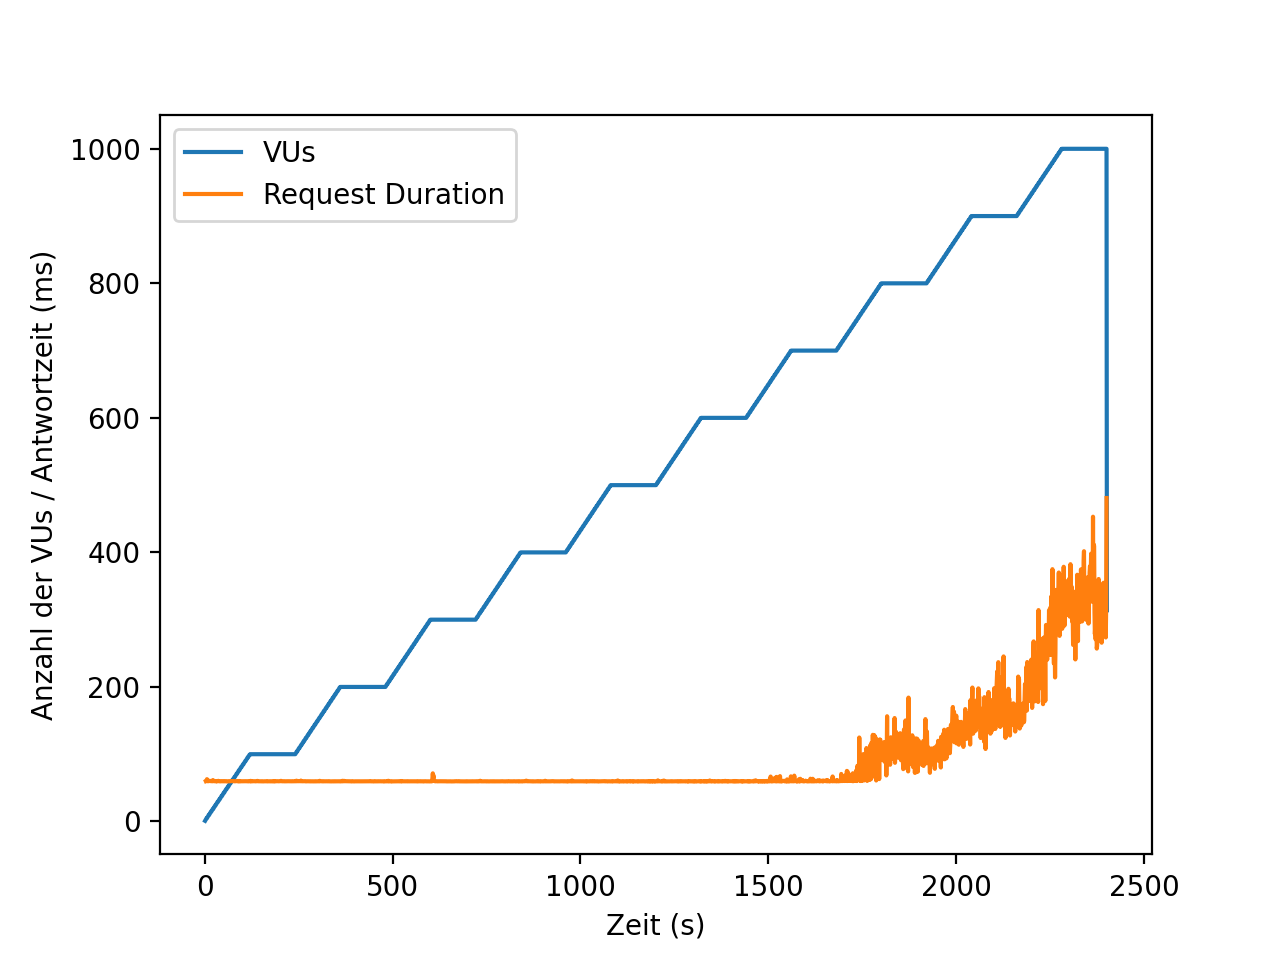
\includegraphics[width=\textwidth]{img/fargate128-stress1000.png}
    \caption[Container Stress-Test 1000VUs]{128MB Container Stress-Test 1000VUs Use-Case A}
    \label{fig:fargate128-stress1000}
\end{figure}

Der dritte Stress-Test für den 128MB Container wurde mit bis zu 1000 VUs durchgeführt. Abbildung \ref{fig:fargate128-stress1000} zeigt den zeitlichen Verlauf dieses Tests für Use-Case A. Es wird dabei die Anzahl der virtuellen Benutzer und die Antwortzeit im Median pro Sekunde dargestellt. Es wird deutlich, dass die Antwortzeit ab ca. 700 VUs deutlich ansteigt. Dies deckt sich der von AWS Cloudwatch gemessenen CPU-Auslastung von knapp unter 100\% die bei dieser Nutzerzahl gemessen wurde. In den Perioden mit Anstieg der VUS steigt auch die Antwortzeit. In jeder Periode mit konstanten Nutzerzahlen können die Requests besser verarbeitet werden und die Kurve geht leicht herunter. Während des Tests wurden trotz einer CPU-Auslastung von teilweise 100\% nur 31 HTTP 502 Fehlercodes vom Server ausgelöst, was einer Quote von 0,0027\% entspricht. Die Antwortzeit konnte im Median weiterhin bei etwa 60ms gehalten werden; die durchschnittliche Antwortzeit stieg mit 116,8ms auf fast das doppelte des Grundwertes an.  
Bei Use-Case B lag die erreichte Prozessor-Auslastung bei 93,14\%. So wurden keine deutlichen Abweichungen ausgelöst. Der Variationskoeffizient stieg mit 0,2 leicht an, liegt aber immer noch deutlich unter dem Wert des Pipe-Clean Tests der 128MB Lambda Funktion. Dieser Wert könnte allerdings auch durch die von den aufgetretenen Fehler verursachten geringen Antwortzeiten gestiegen sein. Diese sind in allen Tabellen-Abbildungen mit einem Stern (*) gekennzeichnet.
Um die maximale Auslastung des Containers für die anderen beiden Use-Cases zu erreichen, wurden noch weitere Stress-Tests mit bis zu 1.500 VUs durchgeführt. Bei Use-Case B konnte das Limit bei ca. 1.100 Benutzern erreicht werden. Für Use-Case C liegt es bei ca. 1.200-1.300 Benutzern.

\subsubsection{Lambda}
Nachdem die maximale Performance des 128MB Containers ermittelt wurde, werden im Anschluss die gleichen Stress-Tests für die Lambda-Anwendung mit 128MB durchgeführt. Abbildung \ref{fig:lambda128-stress-comparison} zeigt die Ergebnisse. 
Allgemein liegt die Antwortzeit im Median immer noch deutlich über der des 128MB Containers; die Differenz ist allerdings im Vergleich zu den Pipe-Clean Tests von 41,74ms auf 16.92ms gesunken (Use-Case A).
Für Use-Case A lässt sich erkennen, dass die Standardabweichung bei 200 und 600 VUs noch um die 19 beträgt, während bei 1000 Usern auf fast 55 ansteigt. Dies könnte allerdings an den extrem langen maximalen Antwortzeiten von bis zu 29.037ms liegen, die durch die Fehler verursacht werden. Die großen Fehler-Latenzen stehen im Gegensatz zu der Container Anwendung, bei der die maximale Antwortzeit immer noch knapp unter einer Sekunde lag. Auffallend ist, dass Fehler mit HTTP Statuscode 500 etwa 10s Antwortzeit aufweisen, während Fehler mit HTTP Statuscode 504 die fast 30s lange Latenz erzeugen. Die bei der Container-Anwendung erzeugten HTTP 502 Fehlercodes, führen stattdessen zu  Antwortzeiten von 12ms bis zu 260ms. 

\begin{figure}[H]
    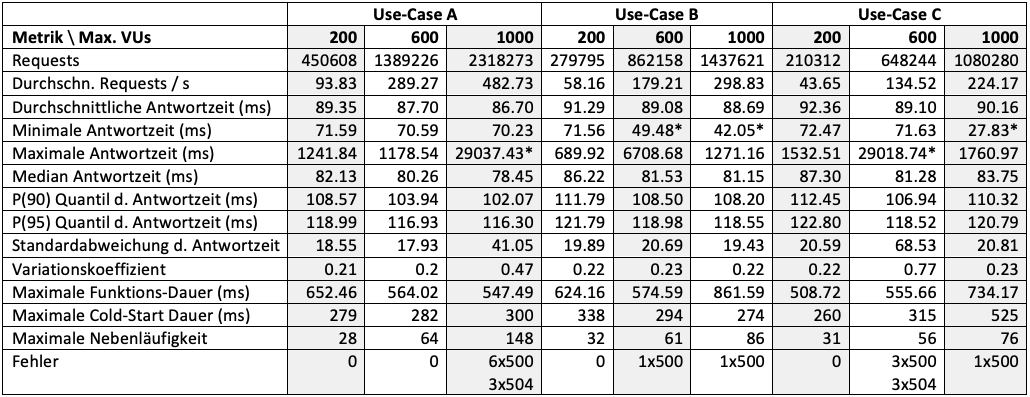
\includegraphics[width=\textwidth]{img/lambda128-stress-comparison.png}
    \caption[Lambda 128MB Stress-Test Vergleich]{Lambda 128MB Stress-Test Vergleich}
    \label{fig:lambda128-stress-comparison}
\end{figure}

Bei der Durchführung der Stress-Tests für die 128MB Lambda-Anwendung fällt außerdem auf, dass die Antwortzeit im Median bei steigenden Nutzerzahlen zu sinken scheint. Bei bis zu 200 VUs lag sie für Use-Case A noch bei 83.65ms, während sie bei bis zu 1000 VUs auf 77.89ms sank. Die Werte für Use-Case B scheinen einem ähnlichen Prinzip zu unterliegen. Es ist jedoch aktuell nicht bekannt, warum dies der Fall ist. Vermutlich provisioniert AWS die Funktionen schneller je mehr Anfragen sie erhalten.
Dies würde auch den Verlauf aus Abbildung \ref{fig:lambda128-stress1000-comparison-graph} erklären, bei dem die drei Use-Cases für den Test mit bis zu 1.000 Benutzern abgebildet sind.

\begin{figure}[H]
    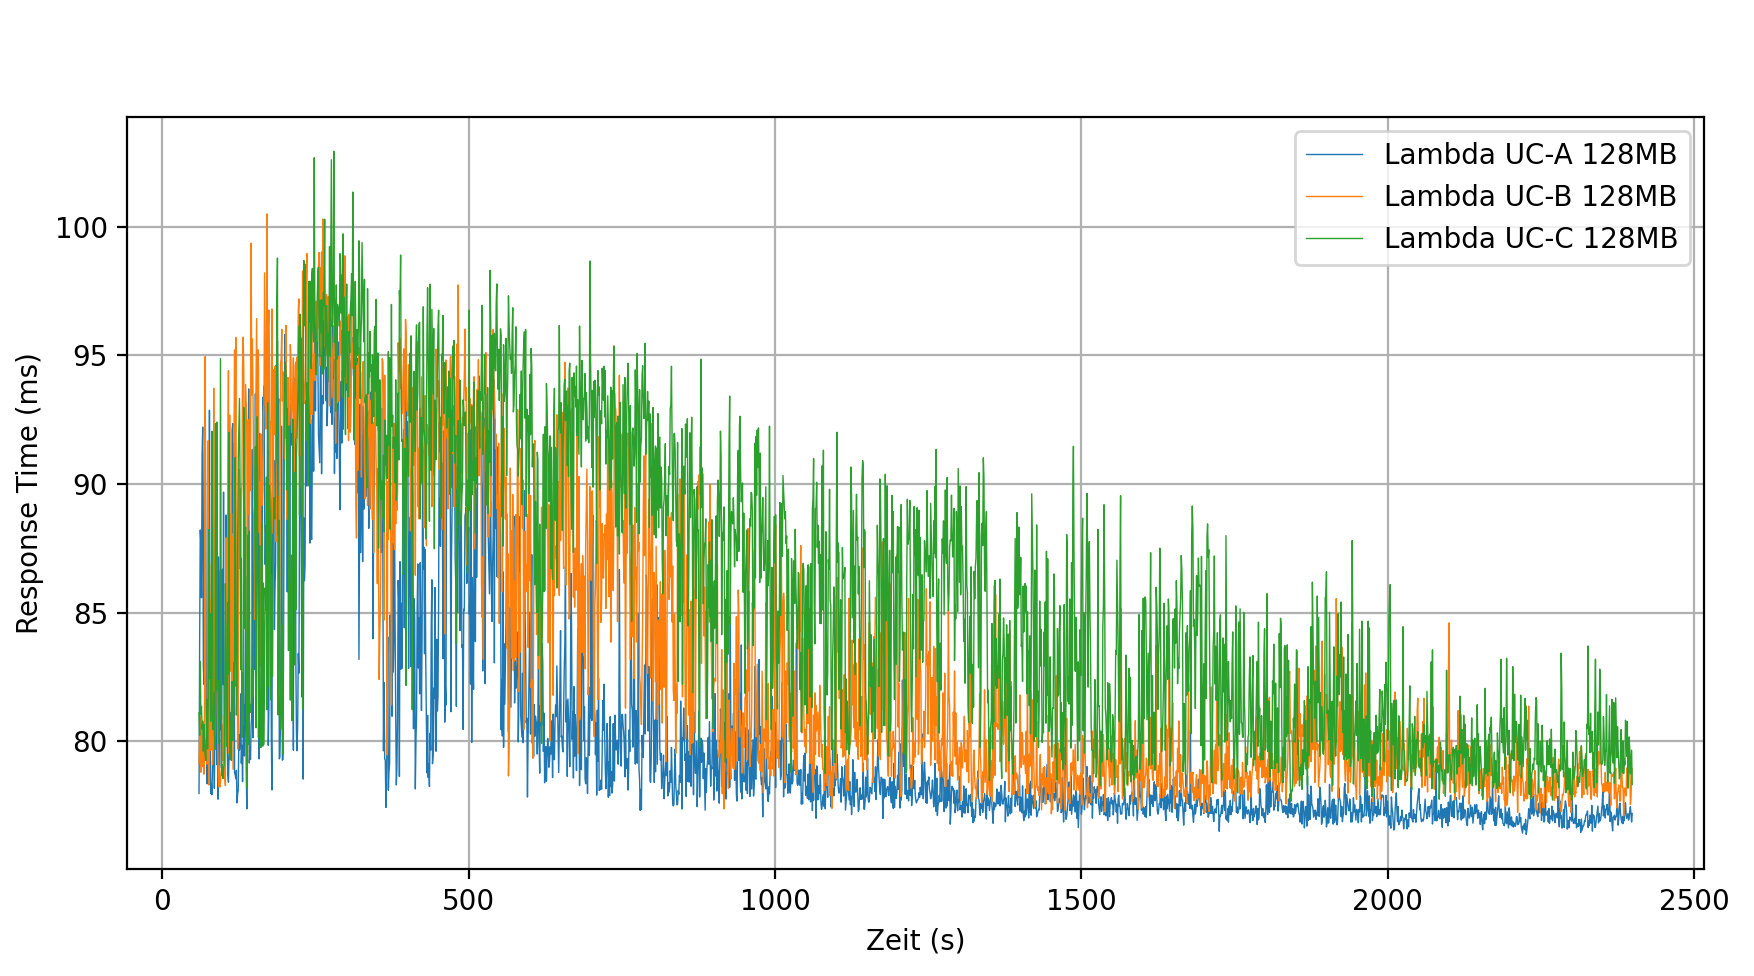
\includegraphics[width=\textwidth]{img/lambda128-stress1000-comparison-graph.png}
    \caption[Lambda 128MB Stress-Test Verlauf Vergleich]{Lambda 128MB Stress-Test Verlauf Vergleich}
    \label{fig:lambda128-stress1000-comparison-graph}
\end{figure}

Aus Gründen der Übersichtlichkeit wurde der Graph erst ab einer Minute dargestellt. Es ist zu erkennen, dass die Antwortzeit bei allen Use-Cases am Anfang ansteigt und nach ca. 300 Sekunden ihren Höhepunkt bei in etwa 95ms bis 100ms erreicht. Danach flachen alle Kurven langsam ab, bis sie ca. 80ms erreichen. Dabei scheint die Kurve von Use-Case A jedoch schneller als die von Use-Case B abzuflachen. Und auch dieser befindet sich schneller auf einem niedrigeren Niveau als der dritte Use-Case.

Zwischen den Use-Cases wird ebenfalls ein Unterschied in der Anzahl der nebenläufigen (concurrent) Lambda-Funktionen deutlich. Während bei 200 und 600 VUs für Use-Case B noch mehr Funktionen bereitgestellt wurden als für Use-Case A, zeigt sich für 1000 VUs ein umgekehrtes Bild. In diesem Fall, übertrifft der erste Use-Case den zweiten um 7 nebenläufige Funktionen. Dies ist interessant gegenüber RQ5, da es der Hypothese widerspricht, dass bei einer einzelnen angefragten Funktion weniger Coldstarts durchgeführt werden müssen als bei mehreren Funktionen (H5). Grund dafür ist vermutlich jedoch die geringere Anzahl der Requests pro Sekunde bei Use-Case B. 

\subsection{Load-Tests}
Für RQ2 soll die Performance unter normalen Nutzerzahlen mit der von schnell ansteigenden Nutzerzahlen verglichen werde. Dazu wird zunächst ein Load-Test für die in den vorangegangenen Stress-Tests ermittelten Nutzer-Grenzen der Container-Anwendung durchgeführt. Im Anschluss wird ein Spike-Test mit der gleichen Benutzerzahl durchgeführt. Ziel dessen ist es, die Performance der Anwendungen unter rasch ansteigender Last zu ermitteln. 

In den bisherigen Stress-Tests wurden nur langsame Anstiege (Ramp-Ups) durchgeführt. Für den Container wurde eine maximale Belastbarkeit von ca. 700 Benutzern ermittelt. Deshalb wird nun für den Load-Test von einem normalem Load von 600 Benutzern ausgegangen. 

\begin{figure}[H]
    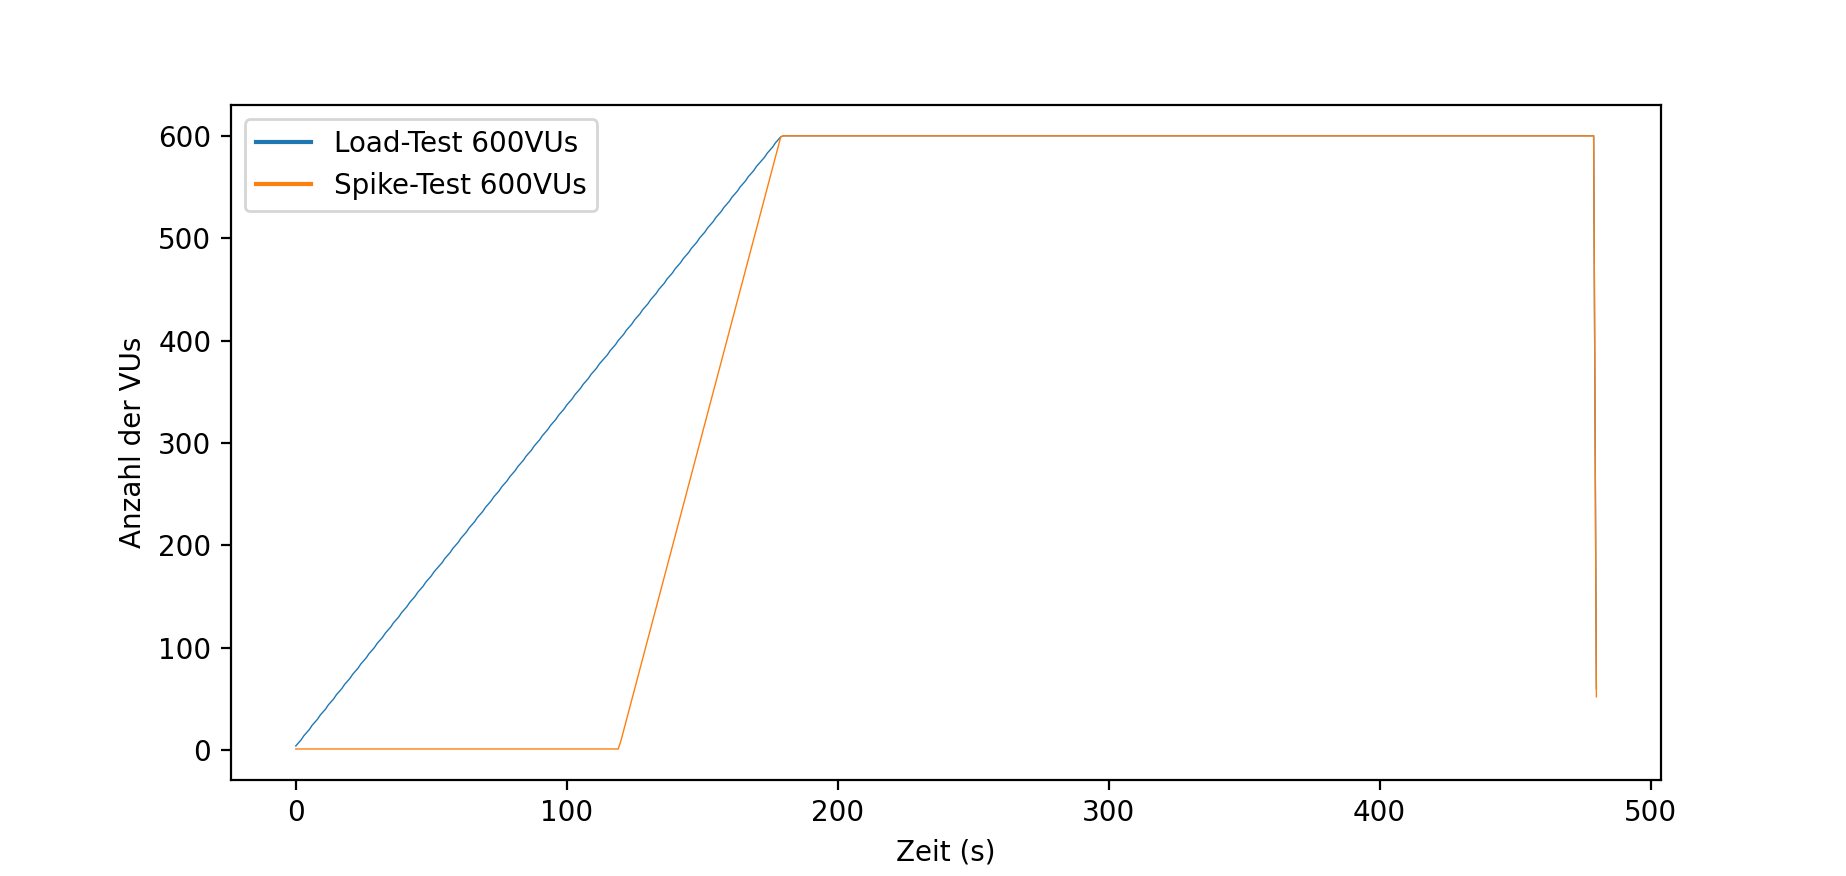
\includegraphics[width=\textwidth]{img/load600-vs-spike600.png}
    \caption[Load- und Spike-Test Vergleich]{Load- und Spike-Test Vergleich}
    \label{fig:load600-vs-spike600}
\end{figure}

Abbildung \ref{fig:load600-vs-spike600} zeigt die unterschiedlichen Test-Verläufe der beiden Tests. Die Anzahl der Benutzer steigt bei dem Load-Test von Anfang an kontinuierlich an und erreichen innerhalb von drei Minuten die maximale Grenze. Für den Spike-Test soll nach einer zwei-minütigen Warte-Phase, in der keine Benutzer auftreten, ein schneller Anstieg innerhalb von einer Minute auf die 600 Virtuelle Benutzer erfolgen. Der Anstieg des Spike-Tests ist also drei mal steiler als der des Load-Tests. 
Nach Erreichen der Obergrenze wird bei beiden Tests die Anzahl der Benutzer für fünf Minuten konstant gehalten. Dies lässt eventuelle Nachwirkungen des Skalierungsverhaltens der Lambda-Funktionen erkennen.


\subsubsection{Container}
Bei der Durchführung der Tests für den 128MB Container konnten keine Veränderungen der Performance für einen schnellen Anstieg der Benutzer gegenüber dem langsamen Anstieg festgestellt werden.

\subsubsection{Lambda}
Bei den Lambda-Funktionen lassen sich für Use-Case A keine eindeutigen Unterschiede in der Antwortzeit für die beiden verschiedenen Anstiegs-Intervalle feststellen. 


\begin{figure}[H]
    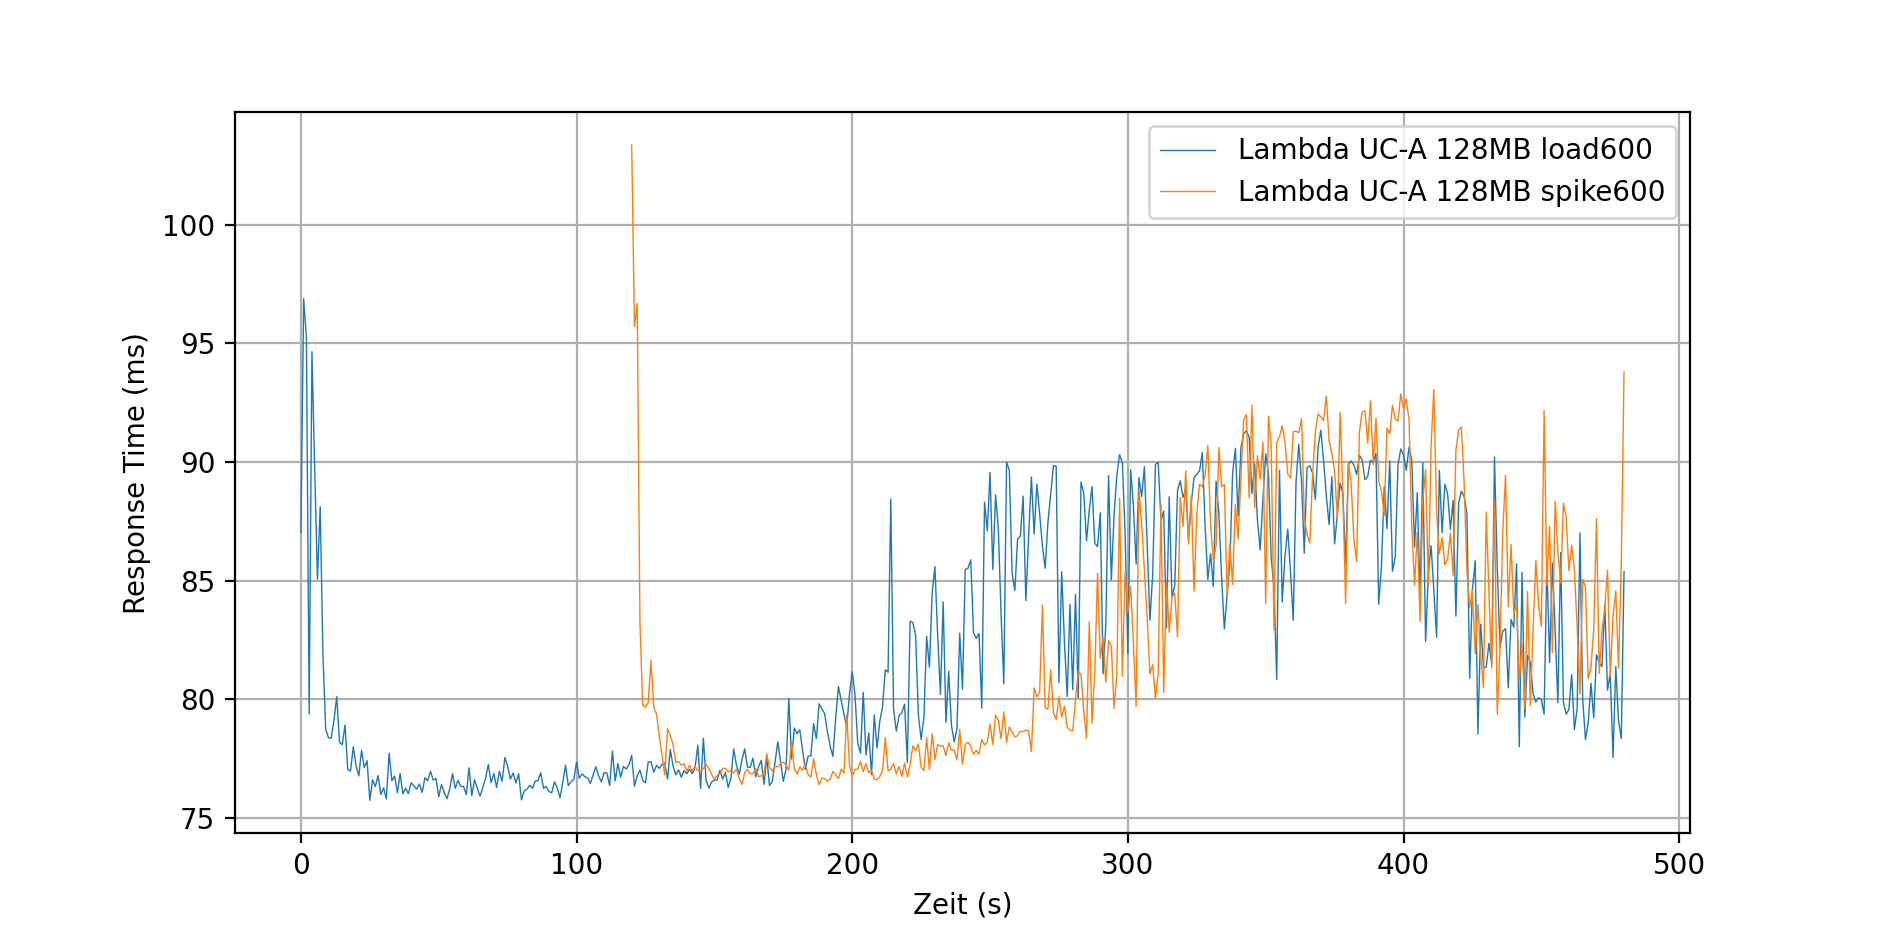
\includegraphics[width=\textwidth]{img/lambda-uca-load600-vs-spike600-example.png}
    \caption[Lambda Use-Case A Load- und Spike-Test Vergleich]{Lambda Use-Case A Load- und Spike-Test Vergleich}
    \label{fig:lambda-uca-load600-vs-spike600-example}
\end{figure}

Abbildung \ref{fig:lambda-uca-load600-vs-spike600-example} zeigt ein Vergleich zweier Load- und Stress-Tests für Use-Case A. Für den Load-Tests (blaue Linie) ist zu erkennen, dass sich nach anfänglich hohen Antwortzeiten von ca 95ms das Niveau bei 75ms - 80ms einpendelt. Ab 180 Sekunden (3 Minuten) ist die maximale User-Anzahl erreicht. Nach ca. 200 Sekunden überschreitet die Median-Antwortzeit für den Load-Test die 80ms Marke und erreicht ihren Höchststand nach ca. 350 Sekunden mit ca. 90ms. Danach sinkt die Median-Antwortzeit wieder trotz konstanter Nutzerzahlen.
Für den Spike-Test scheint es sich ähnlich zu verhalten. Auch wenn nach 180 Sekunden die 600 VUs erreicht wurden, klettert die Antwortzeit allerdings erst mehr als eine Minute später über die 80ms Marke. Der Spike-Test erreicht ebenso wie der Load-Test nach ca. 350 Sekunden sein Maximum; die Antwortzeit liegt mit ca. 93ms nur leicht über der des Load-Tests.

\begin{figure}[H]
    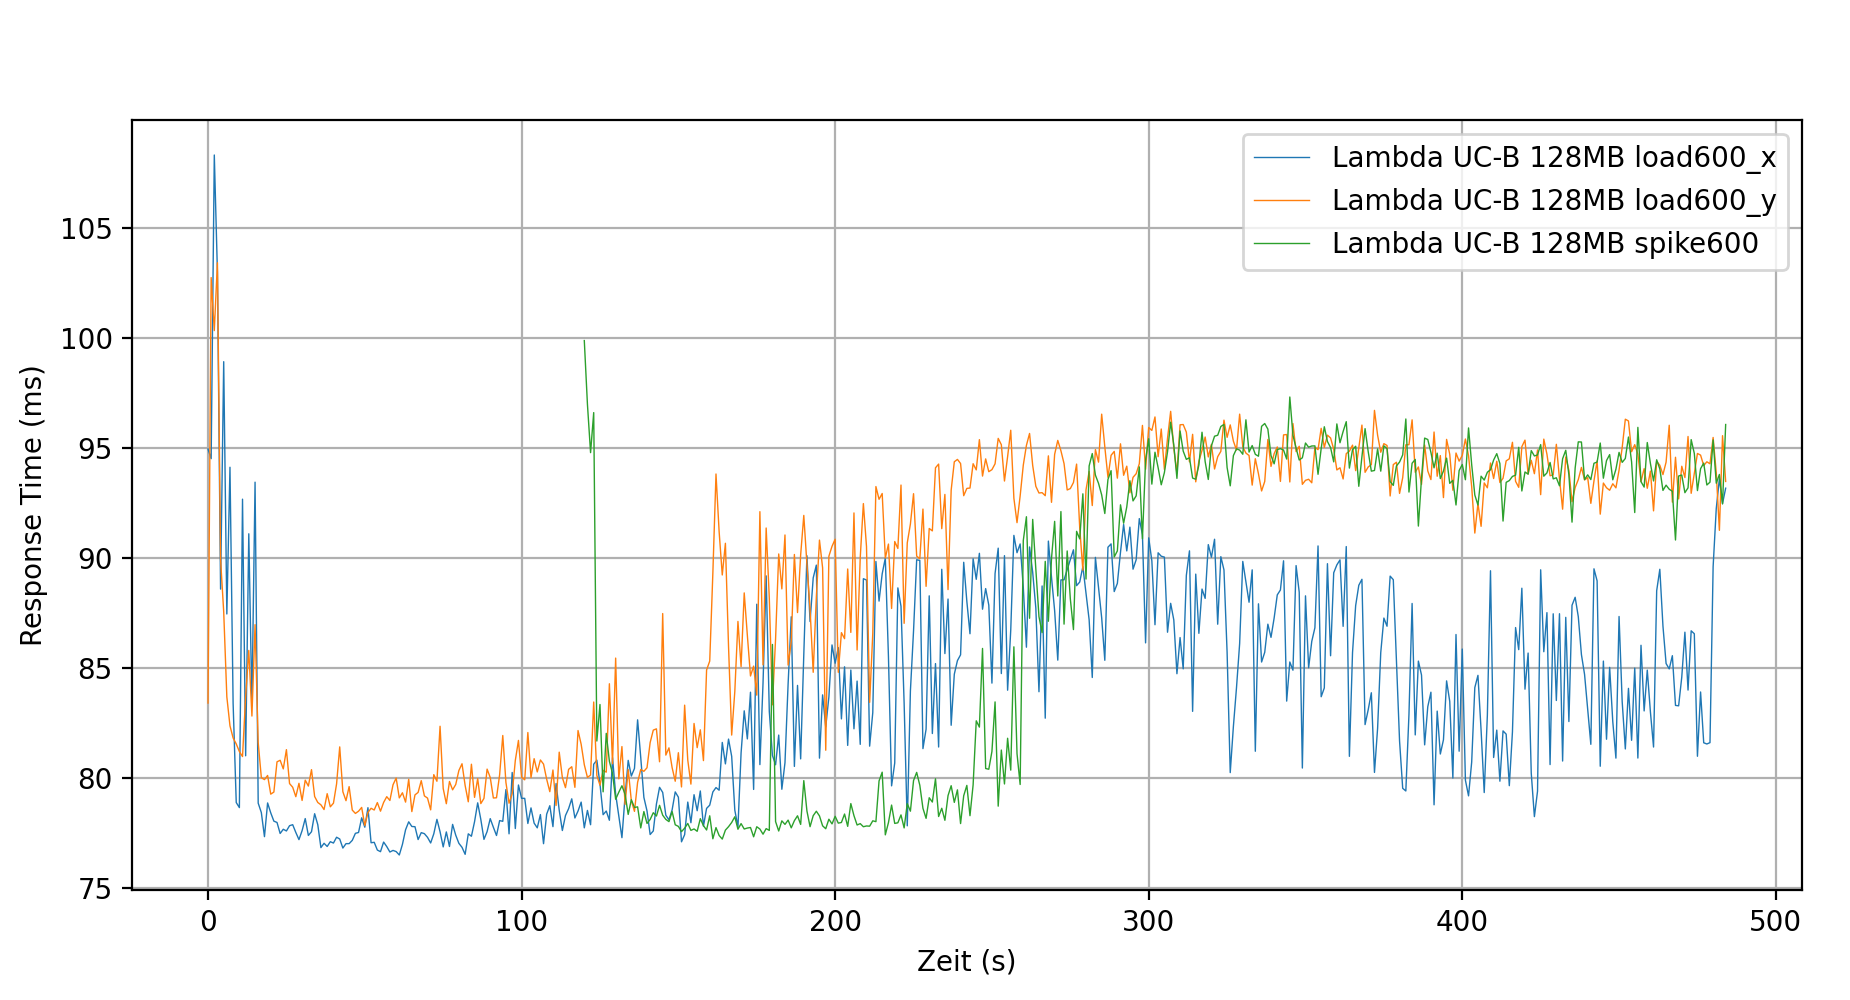
\includegraphics[width=\textwidth]{img/lambda-ucb-load600-vs-spike600-example2.png}
    \caption[Lambda Use-Case B Load- und Spike-Test Vergleich]{Lambda Use-Case B Load- und Spike-Test Vergleich}
    \label{fig:lambda-ucb-load600-vs-spike600-example}
\end{figure}

Für Use-Case B (Abbildung \ref{fig:lambda-ucb-load600-vs-spike600-example}) wurden zwei unterschiedliche Verläufe der Load-Tests festgestellt. Der erste Load-Test (blaue Linie) zeigt einen flacheren Verlauf als der zweite (orange Linie). Seine Kurve fällt nach Erreichen der höchsten Antwortzeit bei ca. 90ms schneller ab. Zudem liegt die maximale Antwortzeit des zweiten Load-Tests mit ca. 95ms in etwa 5ms über der des ersten. Auch der Spike-Test (grüne Linie) erreicht eine maximale Antwortzeit von ca 95ms, womit dessen Verlauf stärker dem zweiten Load Test ähnelt. Es wird deutlich, wie unterschiedlich die Verläufe eines identischen Tests bei der Lambda-Anwendung ausgeprägt sein können. Interessant ist außerdem, dass die Antwortzeit des ersten Load-Test eine größere Schwankung aufweist, als die des zweiten und des Spike-Tests, bei denen aufeinander folgende Werte stets relativ nah beieinander liegen.

Da die Antwortzeiten des Spike-Test trotz des dreimal schnelleren Anstiegs dennoch äußerst nah bei denen der beiden Load-Tests liegen, lässt sich entgegen H1 annehmen, dass ein schneller Spike-Load nur eine geringfügige Veränderung der Antwortzeit mit sich bringt. 

Es zeichnet sich wie auch schon bei den Stress-Tests ein Unterschied der Antwortzeiten zwischen den einzelnen Use-Cases ab. Exemplarisch zeigt Abbildung \ref{fig:lambda128-load600-uc-comparison} den Verlauf der Antwortzeiten im Median für den Load-Test mit bis zu 600 VUs.

\begin{figure}[H]
    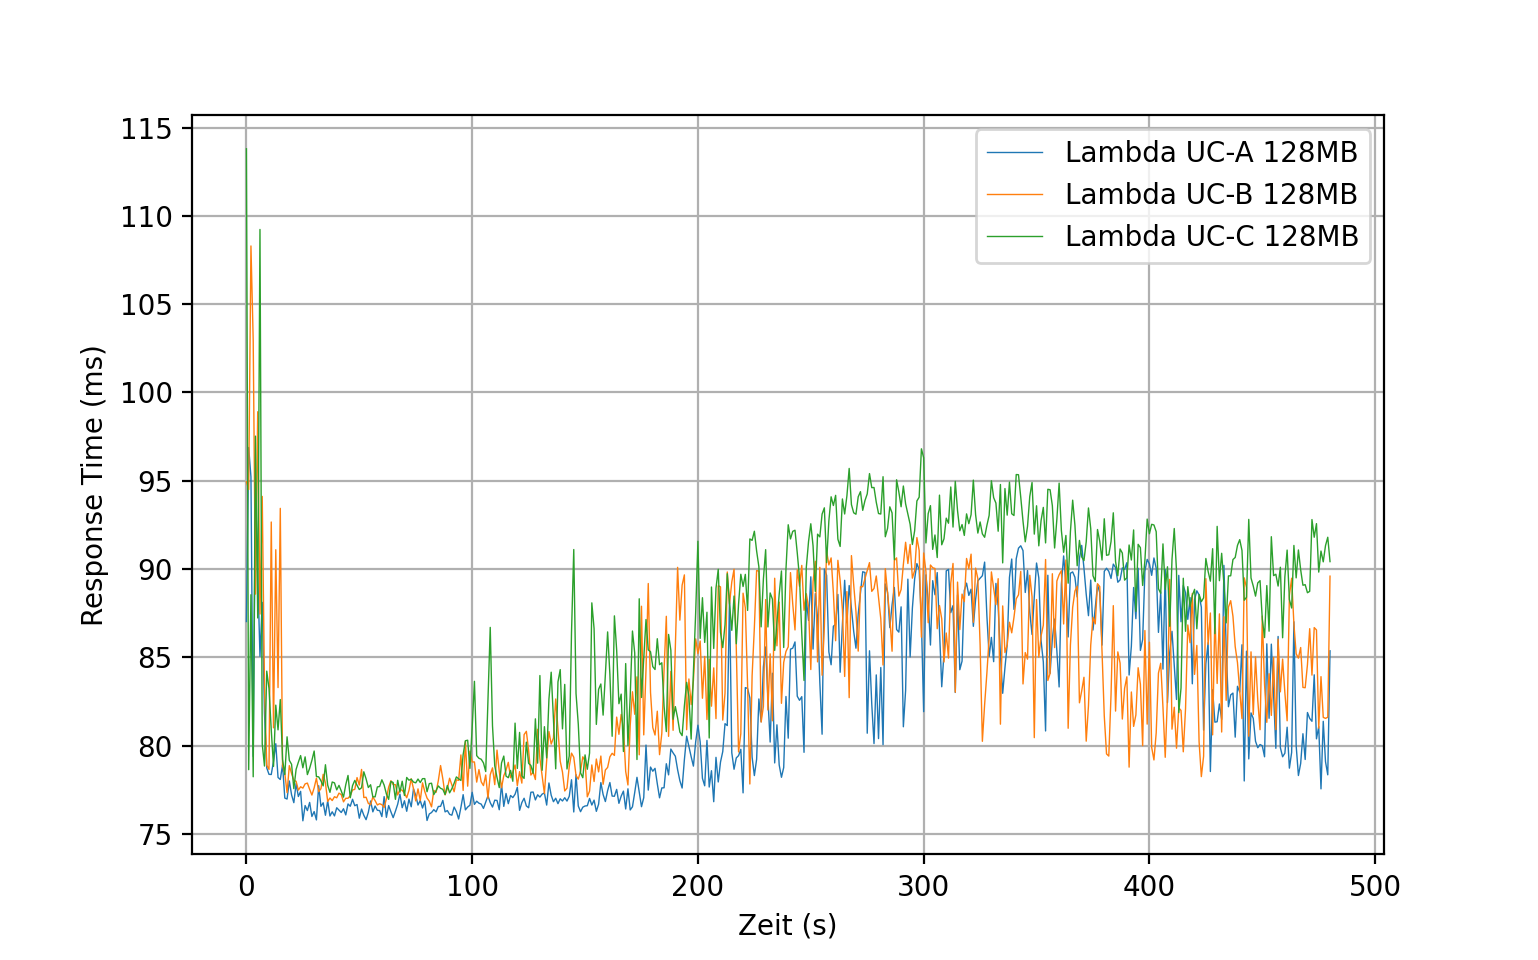
\includegraphics[width=\textwidth]{img/lambda128-load600-uc-comparison.png}
    \caption[Vergleich der 600VU Load Tests für Lambda]{Vergleich der 600VU Load Tests für Lambda}
    \label{fig:lambda128-load600-uc-comparison}
\end{figure}

Es ist zu erkennen, dass alle Use-Cases einen generell ähnlichen Verlauf haben. Use-Case A mit nur einem Endpunkt weist jedoch überwiegend die geringste Antwortzeit auf. Die Linie von Use-Case B liegt nur leicht aber eindeutig über der des ersten Use-Case, übertrifft diesen sogar gegen Ende des Vergleichs. Use-Case C mit den meisten Endpunkten weist auch die höchsten Antwortzeiten auf und erreicht mit über 95ms ein in etwa 5ms höheres Maximum als die anderen beiden Use-Cases.  


\section{Andere Konfigurationen (RQ3)}
Als nächstes sollen Container und Lambda-Funktionen mit einer CPU- und Speicher-Größe von 256 und 512 Megabyte untersucht werden. Ziel dessen ist es, Unterschiede zu den in der vorangegangenen Sektion getesteten Konfigurationen zu erkennen.

\subsection{Pipe-Clean Tests}
Für die Pipe-Clean Tests der Container konnte keine Veränderung zur 128MB Variante festgestellt werden. Die Antwortzeit bewegte sich im Median erneut um die 60ms und auch der Variationskoeffizient zeigte mit ca. 0,01 auch kaum eine Veränderung.
Abbildung \ref{fig:pipe-comparison} zeigt die Pipe-Clean Tests der unterschiedlich großen Konfigurationen der Lambda Funktion für die Use-Cases A und B.

\begin{figure}[H]
    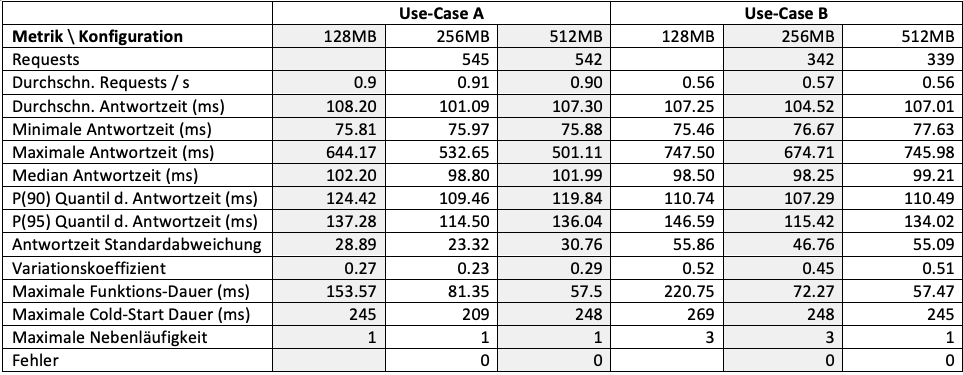
\includegraphics[width=\textwidth]{img/pipe-comparison.png}
    \caption[Vergleich der Pipe-Clean Tests für Lambda]{Vergleich der Pipe-Clean Tests für Lambda}
    \label{fig:pipe-comparison}
\end{figure}

Es wird deutlich, dass auch hier fast keine Unterschiede zwischen den drei Ausführungen bestehen. Die mediane Antwortzeit liegt für alle Use-Cases in etwa bei 100ms. Die P(90) und P(95) Quantile variieren leicht zwischen den Tests der verschiedenen Konfigurationen. Tendenziell sind sie bei den größeren Konfigurationen niedriger als bei den kleineren, es lässt sich jedoch kein eindeutiges Muster erkennen. Es können außerdem keine Unterschiede in der Coldstart-Dauer oder der Varianz festgestellt werden. 
Allerdings ist zu erkennen, dass die maximale Funktionsdauer bei den größeren Konfigurationen deutlich geringer wird und sich dem minimalen Wert von 50ms annähert. Während der Wert für Use-Case A und die 128MB Funktion noch bei 153.57ms liegt, sinkt er für die 256MB Funktion auf nur noch 81.35ms herab. Für die 512MB Variante liegt der Wert nur noch knapp über 60ms. Ähnliches ist für die anderen beiden Use-Cases festzustellen. 

\subsection{Stress- und Load-Tests}
Unter Annahme von H3 wird davon ausgegangen, dass der Container 256MB Speicher und CPU-Größe doppelt so viele Anfragen verarbeiten kann wie der Container mit 128MB. Da der kleinere Container bis zu 700 Benutzer bedienen konnte, wurde im folgenden ein Stress-Test mit bis zu 1500 Benutzern durchgeführt, für den Fall dass er mehr als doppelt so viel verarbeiten kann.
Trotz des doppelt so großen Speichers und vCPUs konnte jedoch keine Verbesserung der maximalen Benutzer für die Container-Instanz erreicht werden. Genau wie der 128MB Container begann die Antwortzeit des 256MB Containers für Use-Case A bei ca. 700 VUs stark anzusteigen. Für Use-Case B kam es ab ca. 900-1.100 VUs zu Anstiegen der Antwortzeiten. Für Use-Case C wurde ein Limit von ca. 1100-1300 VUs erkannt. Damit ist kein wirklicher Unterschied zu der 128MB Variante erkennbar. Die Hypothese H3 kann also für diesen Fall nicht bestätigt werden.

Der Verlauf der Stress-Tests für der 128MB Serverless-Anwendung zeigte, dass eine größere Anzahl an Endpunkten zu höheren Antwortzeiten führen könnte (vgl. Abbildung \ref{fig:lambda128-stress1000-comparison-graph}). Wie Abbildung \ref{fig:lambda256-stress1000-comparison-graph} für den Stress-Test mit bis zu 1000 VUs zeigt, ist dies auch bei den 256MB Funktionen der Fall. Allerdings scheint der Größenunterschied zwischen den Use-Cases im Vergleich zu der kleineren Konfiguration zurückgegangen sein. Auch bei dieser Abbildung werden die ersten 60 Sekunden nicht angezeigt, da die initial sehr hohen Antwortzeiten die Darstellung der Verläufe stark verzerren würde. 

\begin{figure}[H]
    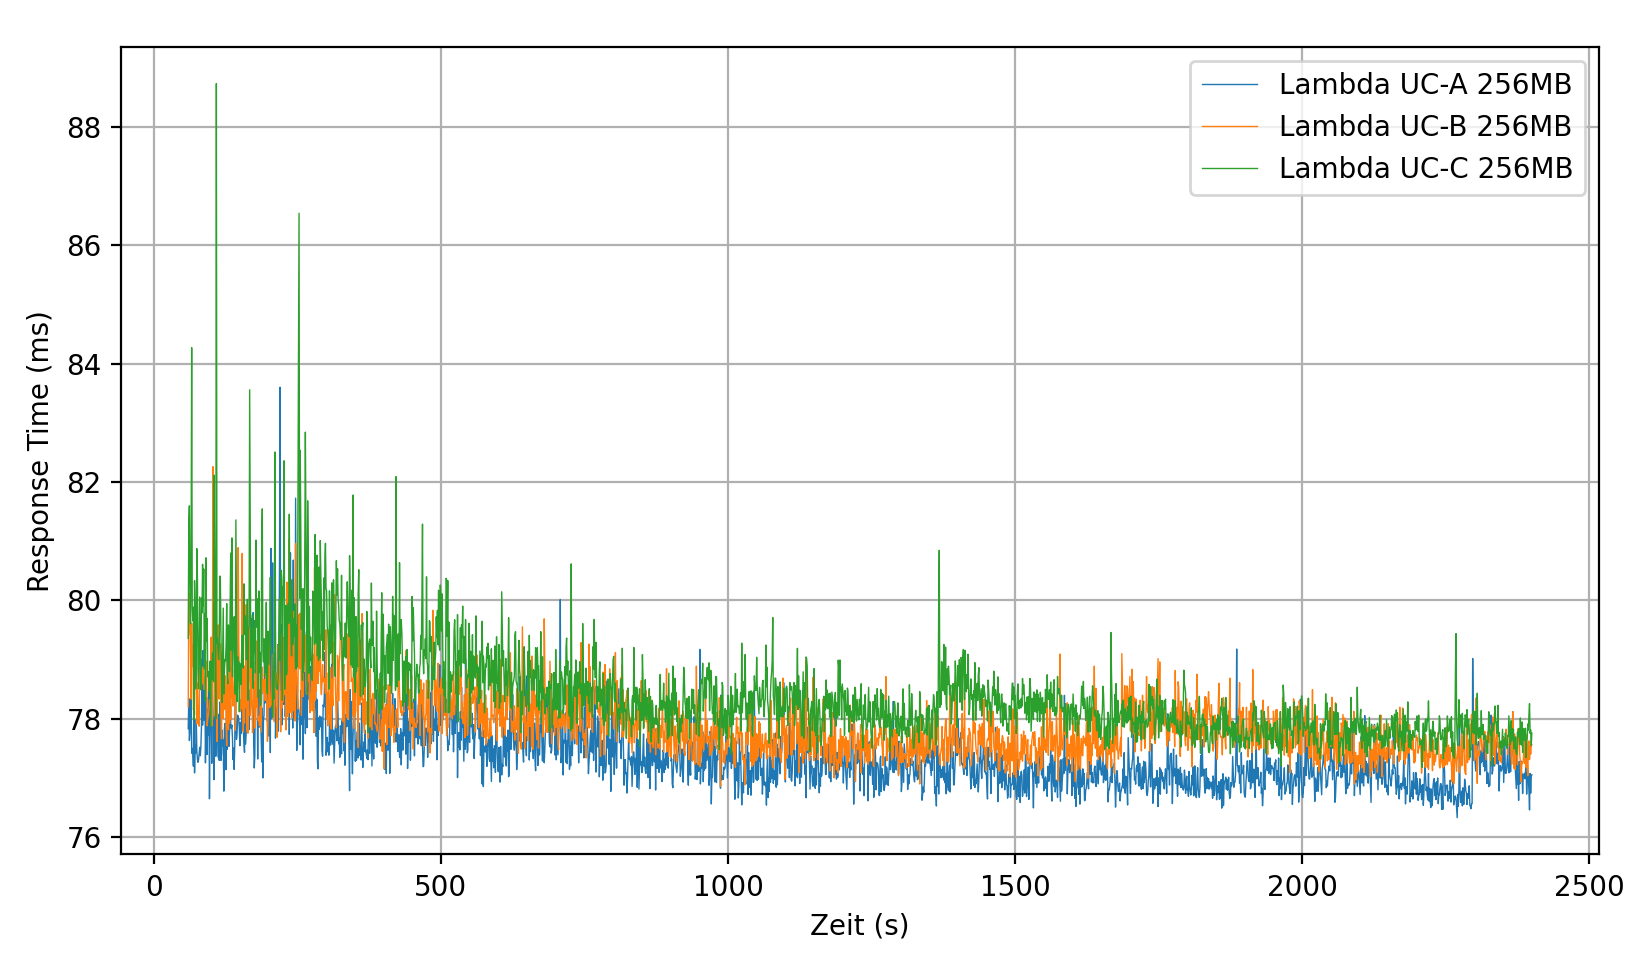
\includegraphics[width=\textwidth]{img/lambda256-stress1000-comparison-graph.png}
    \caption[Lambda 256MB Stress-Test Verlauf Vergleich]{Lambda 256MB Stress-Test Verlauf Vergleich}
    \label{fig:lambda256-stress1000-comparison-graph}
\end{figure}

Bei allen drei Use-Cases lagen die Antwortzeiten dennoch nahe um einen Median-Wert von ca. 78ms und es wurden 95 Prozent aller Anfragen in etwa 100ms verarbeitet. Bei der 128MB Variante reichte das P(95) Quantil noch von 114ms bis zu mehr als 122ms. Der Variationskoeffizient lag ebenso in allen Fällen bei 0,16 bis 0,18 und ist damit deutlich geringer als bei der kleineren Konfiguration, bei der er meistens bei 0,22 lag, allerdings auch einen Wert von 0,64 erreichte. Damit ist eine deutliche Verbesserung der Performance und der Varianz in den Stress-Tests für die 256MB Variante festzustellen.

Im Anschluss wurden die Last- bzw. Spike Tests durchgeführt, um diese mit der 128MB Variante zu vergleichen. Als VU-Limit wurde erneut 600 festgelegt. Dies ermöglicht einen einfachen Vergleich der beiden Varianten.
Auch hier konnte für die Container-Anwendung keine Unterschiede zu der kleineren Konfiguration festgestellt werden. 

\begin{figure}[H]
    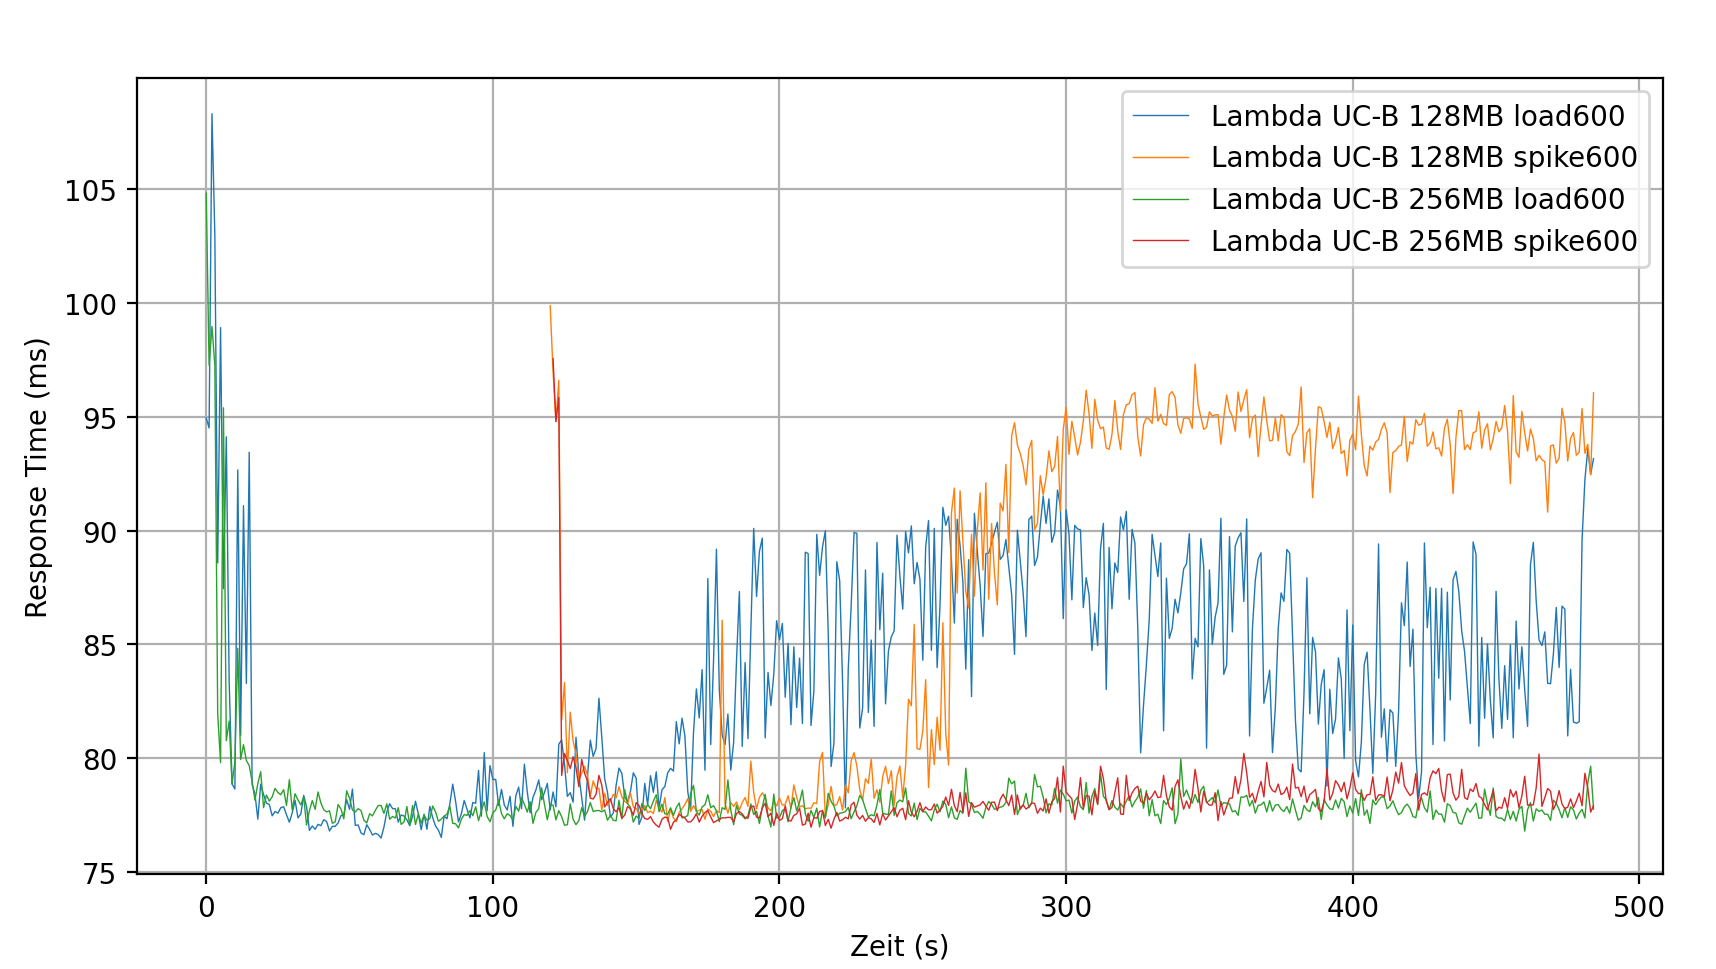
\includegraphics[width=\textwidth]{img/lambda128+256-ucb-load600-vs-spike600-graph.png}
    \caption[Lambda 128MB und 256MB Vergleich der Load- und Spike-Tests]{Lambda 128 und 256MB Vergleich der Load- und Spike-Tests}
    \label{fig:lambda128+256-ucb-load600-vs-spike600-graph}
\end{figure}

Für die Lambda-Funktionen der Use-Cases A und B sind bei der 256MB Variante im Gegensatz zu der 128MB Konfiguration keine wesentliche Unterschiede zwischen den Load- und Spike Tests zu erkennen. Wie in Abbildung \ref{fig:lambda128+256-ucb-load600-vs-spike600-graph} für Use-Case B zu erkennen ist, sind die größeren Funktionen nahezu gar nicht von der Skalierung betroffen. Die Antwortzeit liegt, bis auf den anfänglichen Anstieg, beständig zwischen ca. 75 und 80ms. Im Vergleich zu der kleineren Variante, verkleinerte sich auch hier der Variationskoeffizient von 0,22 auf 0,17. Wie schon bei den Pipe-Clean Tests zu sehen war, sinkt auch die maximale Funktionsdauer von über 600ms bei 128MB auf unter 300ms ab. Bei den Antwortzeiten gab es ebenso eine geringfügige Verbesserung. Bei Coldstart-Dauer konnte dagegen keine Veränderung festgestellt werden.
Allein bei Use-Case C gibt es Unterschiede in den Antwortzeiten. Während der Wert des Medians bei den Load-Tests nur etwas über 78ms liegt, liegt er bei den beiden Durchläufen der Spike-Tests bei 88.46 und 84.26ms. Vermutlich ist dies auf vermehrte Coldstarts durch die größere Anzahl an Endpunkten zurückzuführen.


Als nächstes sollen Container und Lambda-Funktionen mit einer CPU- und Speicher-Größe von 512 Megabyte untersucht werden. Ein Stress-Test des Containers mit bis zu 1500 Benutzern, ergab für Use-Case A, dass die Antwortzeit des Containers ab einer VU-Anzahl von ca. 1400 Benutzern deutlich zunimmt. Mit Eintreten der 1400 Benutzer erreichte das Container Cluster ebenso eine CPU-Auslastung von 100 Prozent. Bei einem zweiten Test war dies für Use-Case A allerdings erst ab ca. 1.600 Benutzern der Fall. Für Use-Case B musste ein weiterer Stress-Test durchgeführt werden, da bei 1500 Benutzern nur eine CPU-Auslastung von 58\% erreicht werden konnte. Der zweite Stress-Test wurde mit bis zu 2.500 Benutzern durchgeführt. Bei ca. 2.200-2.400 VUs wurde die maximale Auslastung des Containers erreicht. Ein weiterer Stress-Test mit bis zu 3.000 VUs ergab für Use-Case C ein Limit von ca. 2.800-3.000 Benutzern.

Im Anschluss an die Stress-Tests des Containers wurden diese mit den gleichen Konfigurationen gegen die Lambda-Anwendung durchgeführt. 

Die Load- und Spike-Tests wurden für die 512MB Konfiguration mit 1.200 VUs durchgeführt. Bei dem Fargate-Container konnte wie schon zuvor keine Unterschiede zwischen den beiden Tests festgestellt werden. Bis auf einige Ausreißer wurde wie schon bei den kleineren Konfigurationen für alle Use-Cases und für beide Anstiege eine Antwortzeit im Median von ca. 60ms festgestellt. Der Variationskoeffizient bewegt sich in den Testausführungen meist zwischen 0,03 und 0,05 und liegt damit nur geringfügig über den Werten der Pipe-Clean Tests. Bis auf eine höhere Anzahl der verarbeitbaren Anfragen konnten also keine Performance-Verbesserungen der 512MB Konfiguration festgestellt werden.

Die Load-Tests der 512MB Lambda-Funktionen bestätigten erneut, dass die Anzahl der Endpunkte einen Einfluss auf die Antwortzeiten hat. Es gab hier allerdings bei den Use-Cases A und B Unterschiede von einigen Millisekunden zwischen den Ausführungen des gleichen Use-Cases. So war die beste Ausführung des Use-Case B besser als die schlechtere Ausführung des Use-Cases A. Die beste Variante des ersten Use-Cases war aber erneut besser als die performanteste Ausführung von Use-Case B. Der Use-Case mit den meisten Endpunkten schnitt auch hier wieder deutlich am unperformantesten ab.

Auch bei den Spike-Tests traten ähnliche Abweichungen wie bei den Load-Tests auf. Deshalb werden für die Analyse nur die jeweils besten Läufe betrachtet. Abbildung \ref{fig:lambda512-load1200-vs-spike1200-graph} zeigt den Verlauf der Load-Tests im Vergleich mit den Spike-Tests. 

\begin{figure}[H]
    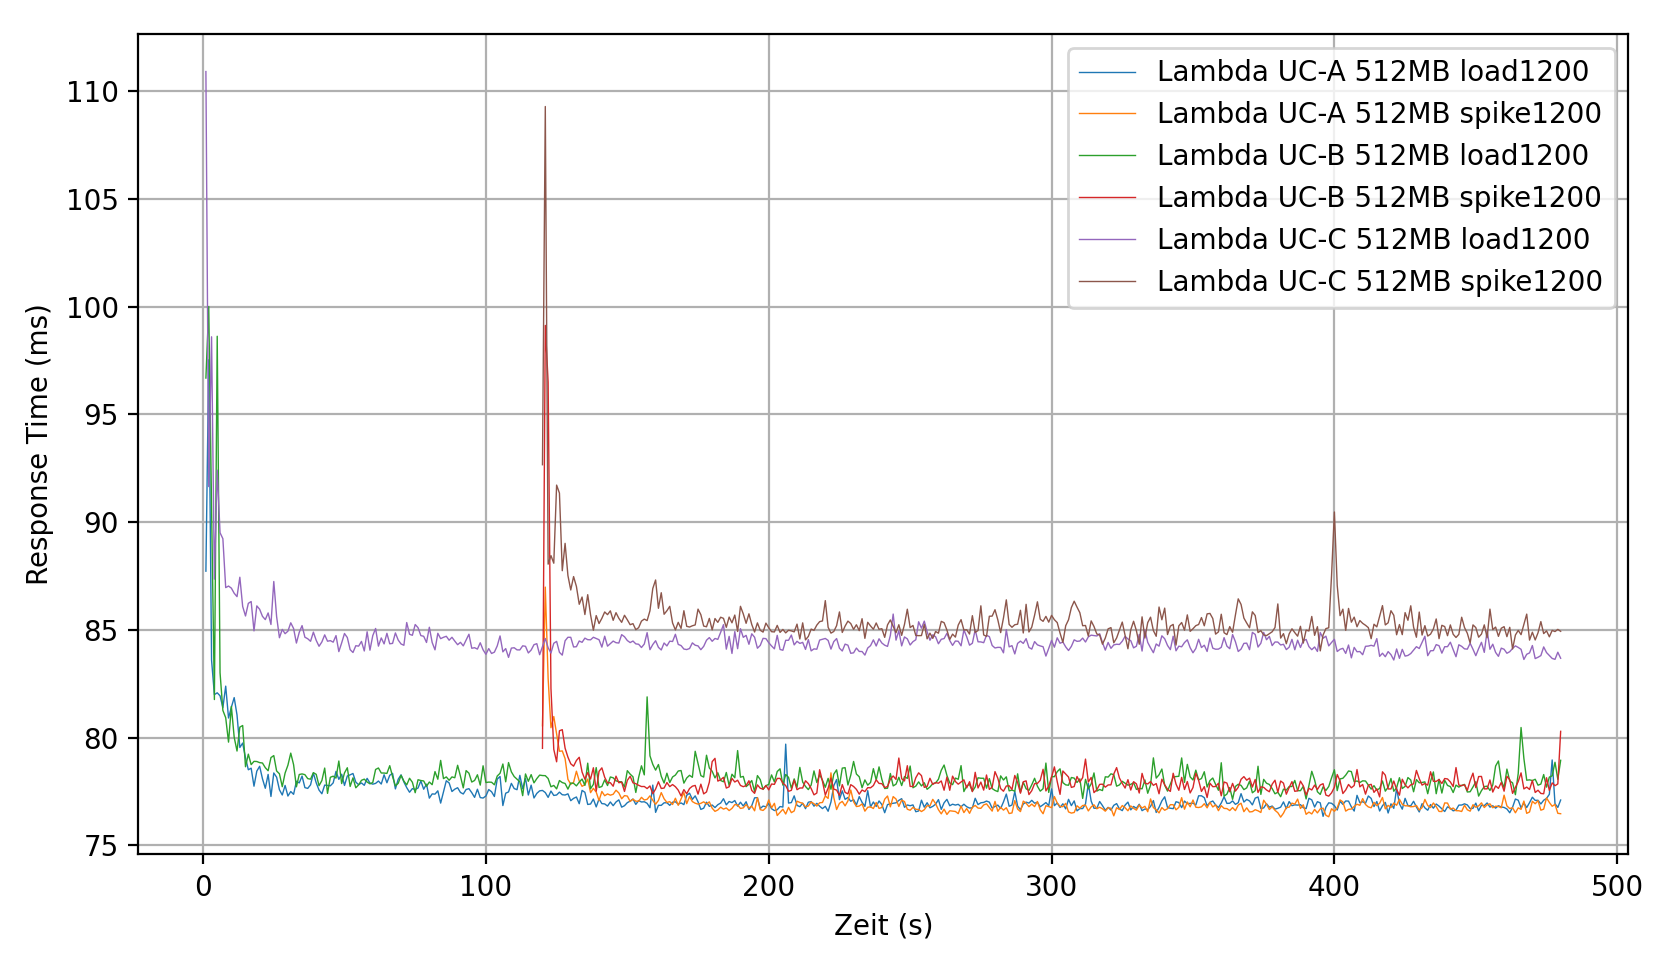
\includegraphics[width=\textwidth]{img/lambda512-load1200-vs-spike1200-graph.png}
    \caption[Vergleich der Lambda 512MB Load- und Spike-Tests]{Vergleich der Lambda 512MB Load- und Spike-Tests}
    \label{fig:lambda512-load1200-vs-spike1200-graph}
\end{figure}

Auch hier zeichnet sich der Einfluss der Anzahl der Endpunkte ab. Der Median von Use-Case B liegt mit 78ms zwar nur knapp über den 77,02ms von Use-Case A. Deutlicher ist aber der Abstand von Use-Case C, dessen Antwortzeiten sich fast durchgängig bei in etwa 85ms befinden. 
Wie schon bei der 256MB Konfiguration ist kein Unterschied zwischen den Load-Test Ausführungen der Use-Cases A und B und den korrespondierenden Spike-Tests erkennbar. Für Use-Case C kann in der 512MB Konfiguration das gleiche beobachtet werden. Es zeigt sich also trotz der doppelt so großen Benutzerzahl im Vergleich zu den kleineren Konfigurationen eine Verbesserung des Skalierungsverhaltens.  

\section{Mehrere Container (RQ4)}
Für die Untersuchung inwiefern sich die Anzahl der aktiven Container auf die Performance auswirkt, wurde ein Test mit der Fargate 256MB Task-Definition durchgeführt. Dazu wurden zwei Container-Instanzen gestartet und den gleichen Stress-Tests unterzogen wie die einzelne 512MB Container-Instanz. Abbildung \ref{fig:fargate-512-vs-2x256-stress-comparison} zeigt das Ergebnis des Tests.

\begin{figure}[H]
    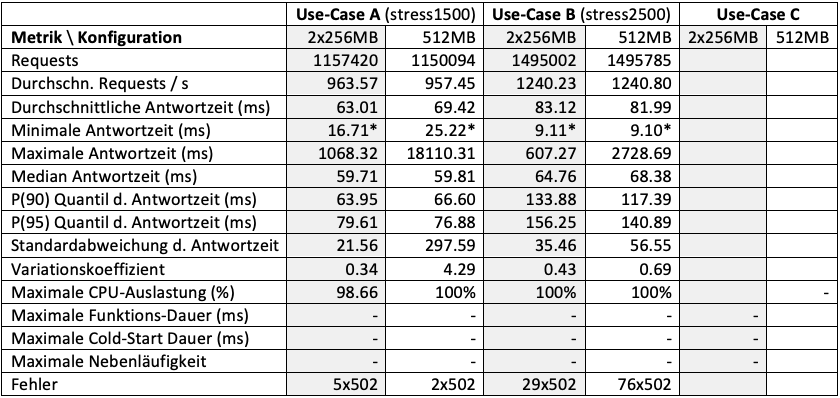
\includegraphics[width=\textwidth]{img/fargate-512-vs-2x256-stress-comparison.png}
    \caption[Vergleich einer 512MB Instanz mit zwei 256MB Instanzen]{Vergleich einer 512MB Instanz mit zwei 256MB Instanzen}
    \label{fig:fargate-512-vs-2x256-stress-comparison}
\end{figure}

In diesem Test wird kein Unterschied in der Performance einer einzelnen 512MB Instanz zu zwei 256MB Instanzen deutlich.


\section{Kosten}
\label{sec:kosten}
In dieser Sektion sollen die Kostenmodelle der in dieser Arbeit getesteten Technologien untersucht und verglichen werden. Dabei wird sich erneut aufs Amazon AWS beschränkt. Es kann daher bei anderen Public-Cloud Anbietern deutliche Unterschiede geben. In AWS gibt es Kostenunterschiede für die einzelnen AWS Regionen. Die folgenden Ausführungen beziehen sich daher ausschließlich auf die Region Frankfurt (eu-central-1).

\subsection{Container}
Da viele verschiedene Wege existieren, Container-Anwendungen in der Public Cloud zu betreiben, wird für die Kosten-Schätzung deshalb nur der Betrieb der Anwendung mit AWS ECS Fargate-Starttyp und Amazon Elastic Kubernetes Service betrachtet.

Bei Fargate wird die Abrechnung in die gewählte Arbeitsspeicher und vCPU-Größe unterteilt. Der Preis für ein Arbeitsspeicher Gigabyte pro Stunde beträgt aktuell 0,00511\$ und der pro vCPU pro Stunde 0,04656\$. Die Formel \ref{fargate-kosten-formel} zeigt die Berechnung der Kosten für ein Fargate-Cluster.


\begin{equation}
Kosten = Tasks * Stunden * Tage * (SpeicherGB * 0,00511\$ + AnzahlvCPUs * 0,04656\$)
\label{fargate-kosten-formel}
\end{equation}

Es wird davon ausgegangen, dass mindestens ein Task dauerhaft laufen muss, damit der Service erreichbar bleibt. Für die in dieser Arbeit verwendete 128MB und 256MB Konfigurationen (mit 0.25 vCPU) ergäben sich für einen laufenden Task pro Monat (30 Tage) und Dauerbetrieb (24 Stunden pro Tag) Kosten von: \\

$Kosten = 1 * 24 * 30 * (0,5 * 0,00511\$ + 0,25 * 0,04656\$) = 10,22\$$ \\

Dieser Wert konnte mit den in dieser Arbeit durchgeführten Tests bestätigt werden, da für jeden Tag Kosten von 0,34\$ für die Nutzung des Clusters von AWS aufgeführt wurden. Bei 30 Tagen Laufzeit ergeben sich damit tatsächlich Gesamtkosten von 10,2\$.

Aus der Formel lässt sich ableiten, dass sich für eine n-fache Anzahl an Tasks auch die n-fachen Kosten pro Monat ergeben. Variationen in der Anzahl der Tasks aufgrund von (Auto-) Skalierung sind schwer vorauszusagen und werden daher nicht berechnet.

Zusätzlich zu den Fargate Kosten sind noch Gebühren für die Nutzung des Load-Balancers fällig, dessen Nutzung bei der Verwendung mehrerer Instanzen unabdingbar ist. Für einen Application Load Balancer fallen pro angefangener Stunde Kosten von 0,027\$ an. Das ergibt für 30 Tage Kosten von 19,44\$. Zusätzlich fallen noch Gebühren für die Auslastung des Load-Balancers an; bspw. für die aktiven Verbindungen pro Minute\cite{noauthor_preise_nodate}. Auch diese können nicht vorausgesagt werden und werden daher bei der Berechnung vernachlässigt.

Die folgende Übersicht zeigt die monatlichen Fixkosten einer Instanz für die unterschiedlichen in dieser Arbeit verwendeten Konfigurations-Größen inklusive Nutzung eines Application Load Balancers:

\begin{itemize}
    \item 128MB = 0,5GB und 0,25 vCPU = 10,22\$ + 19,44\$ (ELB) = 29,66\$
    \item 256MB = 0,5GB und 0,25 vCPU = 10,22\$ + 19,44\$ (ELB) = 29,66\$
    \item 512MB = 1  GB und 0,5  vCPU = 20,44\$ + 19,44\$ (ELB) = 39,88\$
    \item 1024MB = 2 GB und 1    vCPU = 40,88\$ + 19,44\$ (ELB) = 60,32\$
\end{itemize}

\noindent
Kosten für Skalierung und die Nutzung des Load-Balancers sind hierbei noch zu ergänzen. 

\subsection{Lambda}
\label{subsec:kosten-lambda}
Die Ausführung von Lambda-Funktionen wird nach der Ausführungszeit in Millisekunden abgerechnet. Dabei wird die Zeit für einen Cold-Starts mit einberechnet. Auch die konfigurierte Arbeitsspeichergröße fließt mit in das Ergebnis ein. Derzeit berechnet AWS in der Region Frankfurt Kosten von 0,0000166667 US-Dollar pro Gigabyte-Sekunde (GB-Sekunde) \cite{noauthor_lambda_nodate}. Zusätzlich müssen pro 1.000.000 Ausführungen im Monat noch einmal 0,20 US-Dollar Anforderungsgebühren gezahlt werden. AWS bietet ein kostenloses Nutzenkontingent von 400.000 Aufrufen pro Funktion im Monat an.

Für die Ausführung der Lambda-Funktionen wird ein Event-Auslöser für REST-Anfragen benötigt. Dazu wurde in dieser Arbeit Amazon API Gateway verwendet, welches eingehende Requests auf die vorgesehene Lambda-Funktion weiterleitet. Für die Verwendung des API Gateways fallen zusätzliche Kosten an. Bei Nutzung des Serverless Frameworks wird automatisch eine API des Typs REST erstellt. Es fallen für diesen API-Typ Kosten von 3,70 Euro pro einer Millionen Aufruf an. Diese werden für jede API insgesamt gerechnet und gelten damit nicht für jede einzelne aufgerufene Lambda-Funktion. Es gibt Vergünstigungen ab 333 Millionen Aufrufen im Monat. In dieser Arbeit werden keine Caching Mechanismen des API Gateways verwendet. Werden diese in den Einstellungen der API aktiviert, fallen zusätzliche Kosten an. AWS bietet für das API Gateway ein kostenloses Nutzenkontingent von einer Millionen Aufrufen im Monat an\cite{noauthor_amazon_nodate}. Formel \ref{lambda-kosten-formel} zeigt die Berechnung der Gesamtkosten für eine Lambda-Funktion.

\begin{equation}
\begin{split}
Kosten = Aufrufe * \left(\frac{LaufzeitMs}{1000ms} * \frac{FunktionsMb}{1024Mb} * 0,0000166667\$ + \frac{0,20\$ + 3,70\$}{1.000.000}\right)
\end{split}
\label{lambda-kosten-formel}
\end{equation}

In den Tests der vorherigen Kapitel lag die Antwortzeit der Lambda Funktionen im Median oft um einen Wert von ca. 80ms. Unter Nutzung der Kostenformel \ref{lambda-kosten-formel} ergibt sich für eine Millionen Aufrufe einer einzigen Lambda-Funktion mit einer Größe von 128MB und dieser Laufzeit, ohne Einberechnung der kostenlosen Nutzenkontingente, ein Preis von: \\

\noindent
$Kosten = 1.000.000 * \left(\frac{80}{1000}*\frac{128}{1024} * 0,0000166667\$ + \frac{0,20\$ + 3,70\$}{1.000.000}\right) = 4,07\$$ \\

Die nachfolgende Tabelle zeigt die Kosten der unterschiedlichen Funktionsgrößen pro 1.000.000 Aufrufe und für eine Laufzeit von 80ms.

\begin{table}[H]
\label{lambda-kosten-70ms-1000000aufrufe}
\begin{tabular}{lllll}
\hline
Funktionsgröße & 128MB   & 256MB   & 512MB   & 1024MB  \\ \hline
Kosten         & 4,07 \$ & 4,23 \$ & 4,57 \$ & 5,23 \$ \\ \hline
\end{tabular}
\end{table}

Da bei Lambda im  Gegensatz zu ECS/Fargate nur die tatsächlich aktive Zeit der Funktion berechnet wird, lässt sich grob abschätzen, wie viele Funktionsaufrufe zu dem gleichen Preis der Fargate Nutzung von einem Container möglich sind (siehe vorherige Sektion). Es wird davon ausgegangen, dass eine Funktion eine Laufzeit von 1ms bis zu 100ms hat. Die Umstellung der Kostenformel \ref{lambda-kosten-formel} ergibt Formel \ref{lambda-aufrufe-formel} zur Berechnung der Aufrufe bei Angabe der Kosten.

\begin{equation}
\label{lambda-aufrufe-formel}
Aufrufe = \frac{Kosten}{\frac{LaufzeitMs}{1000ms} * \frac{FunktionsMb}{1024Mb} * 0,0000166667\$ + \frac{0,20\$ + 3,70\$}{1.000.000}}
\end{equation}

Abbildung \ref{fig:lambda-max-invocations} zeigt das Ergebnis der Berechnungen. Die Werte der 128MB und 256MB Funktionen stimmen überein, da der Preis für die Fargate Konfiguration identisch ist.

\begin{figure}[H]
    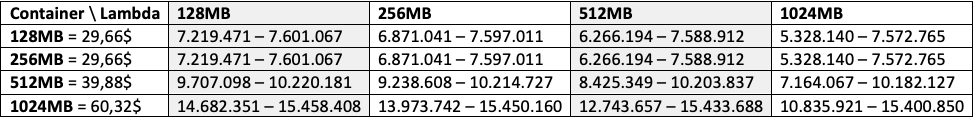
\includegraphics[width=\textwidth]{img/lambda-max-invocations.png}
    \caption[Anzahl der Aufrufe von Lambda-Funktionen dem Monatspreis von Fargate entsprechend]{Anzahl der Aufrufe von Lambda-Funktionen dem Monatspreis von Fargate entsprechend}
    \label{fig:lambda-max-invocations}
\end{figure}

Der jeweils linke Wert in den Tabellenzellen gibt dabei die maximale Anzahl der Aufrufe an, wenn jeder Funktionsaufruf bei 100ms liegt. Der rechte Wert ist der für eine Funktions-Dauer von 1ms und ist damit der maximal mögliche Wert, da Lambda immer mindestens eine Millisekunde abrechnet\cite{noauthor_lambda_nodate}.